\documentclass[10pt,twocolumn,letterpaper]{article}
\usepackage[review]{cvpr}
\usepackage{booktabs}
\usepackage{amsmath,amssymb}
\usepackage{graphicx}
\definecolor{cvprblue}{rgb}{0.21,0.49,0.74}
\usepackage[pagebackref,breaklinks,colorlinks,allcolors=cvprblue]{hyperref}

\def\paperID{*****}
\def\confName{CVPR}
\def\confYear{2027}

\title{A Degree Match Does Not Keep Both Inputs}

\author{Anonymous}

\begin{document}
\maketitle

\begin{abstract}
Connectome-constrained vision models are compared with null graphs that match a degree sequence, a motif count, or a wiring cost.
Under incoming-neighbor averaging, those matches do not say whether both inputs of a computation still reach the readout, or whether they arrive as two directions or as one mixture.
On a 768-neuron visual subgraph of the male fly central nervous system, we keep the four strongest incoming synapses and apply the average twice.
Two edits match the measured graph in edge count, degree sequence, and module-pair counts.
One leaves both source columns nonzero and independent.
The other deletes a column.
The same MLP scores $0.979$ and $0.746$ in the first case, and $0.504$ and $0.506$ in the second.
The measured graph, whose columns are nonzero but parallel, scores $0.976$ on a subspace XOR and $0.663$ on digit parity.
A linear readout stays at chance.
The usual degree-preserving null, ten swaps per edge, retains both columns in none of 24 draws.
At 307 swaps, 11 of 12 draws still retain both columns and a degree match, and the transfer usually changes.
Digit parity on those draws follows the rank of the transfer: five rank-2 draws score between $0.715$ and $0.727$, and six rank-1 draws score between $0.646$ and $0.673$.
The draw that loses a column scores $0.506$.
\end{abstract}

\section{Introduction}
\label{sec:intro}

A measured wiring diagram is a concrete prior for a visual network.
Fly connectomes now make that prior available at synaptic resolution, and models that keep the diagram fixed can predict neural responses and support visual discriminations from the graph alone \cite{lappalainen2024,dorkenwald2024,berg2026,correig2026}.
The same diagrams are also being used as controls.
When a connectome-constrained network is trained from a shared initialization, a degree-preserving rewire can remove an apparent advantage over a weaker random graph \cite{dhiman2026}.
An evolutionary comparison changes in the other direction once the null is forbidden to rewire the sensory-to-motor boundary \cite{park2026}.
Separating the physiology tuned on the real wiring from the physiology retuned on each null changes still other verdicts, including a flyvis ranking and a mushroom-body learning comparison \cite{liu2026}.
These papers agree on a narrower point than their headlines suggest.
The verdict follows the control.

They do not yet agree on what the control has to preserve.
A degree-preserving swap matches the number of inputs and outputs at every neuron \cite{maslov2002}.
A motif count matches a chosen subgraph \cite{milo2002}.
A wiring-cost match constrains how much wire the randomized graph may spend \cite{correig2026}.
None of these statements is a statement about the signal that arrives at a chosen pair of sinks after a stated propagation rule.
For a readout that needs two inputs, that signal is the relevant object.
If a null deletes one input, a drop in accuracy is what the deletion predicts.
It is not evidence that the degree sequence was a sufficient description of the wiring.

This paper measures that object for one propagator and one subgraph.
Each neuron replaces its state by the mean of the neurons that point to it.
Two such steps map a pair of source features to a pair of sinks.
We take the visual neurons of the male central nervous system \cite{berg2026}, keep the 768 neurons of highest total degree, and retain the four strongest incoming synapses at each neuron.
A deterministic search then fixes one relay, its first two inputs, and its first two outputs.
The measured graph and two module-matched edits of that graph share the degree sequence and the module-pair counts.
Only the measured graph still has a relay used by both sources.
One edit leaves both source columns nonzero and linearly independent.
The other deletes a source column.
An MLP fit to the sink state follows this difference.
A linear map of the same state does not, because both tasks are XOR.
Separately, a standard degree-preserving null, run for the usual mixing budget of ten swaps per edge, keeps both sources in none of 24 draws. At 307 swaps both sources remain in 11 of 12 draws, and digit parity follows the rank of the transfer rather than the shared degree sequence.

The observation that matters is empirical, and it is easy to miss if the only reported statistic is a degree sequence or a motif count.
Removing the shared relay can improve a two-input visual readout, and a degree-matched edit that removes one source destroys it.
The certificate that tracks the MLP is the source-column support of the averaged propagator, not the degree match and not the presence of the relay.

\section{Related work}
\label{sec:related}

Connectome-constrained models treat the adjacency as given and learn the quantities the reconstruction does not provide.
Flyvis learns membrane and synapse parameters on the optic-lobe wiring and predicts responses across the visual system \cite{lappalainen2024}.
A connectome-only model passes an eye image through the measured graph and reads Kenyon cells, comparing the biological wiring with randomized graphs at matched cost \cite{correig2026}.
Dhiman revisits an apparent topology gain in a flyvis-style recurrent mask and finds that shared initialization removes the early-loss gap, while a degree-preserving null removes the activity gap \cite{dhiman2026}.
The recurrence there is a masked weight, $W_G = M_G \odot \widetilde W$, not an average over incoming neighbors.
Park shows that column shuffles and degree-preserving swaps create one-step olfactory-to-descending shortcuts that the fly graph almost entirely lacks, and that those shortcuts decide an evolutionary comparison \cite{park2026}.
Liu separates three ways of assigning the unmeasured physiology and shows that some wiring verdicts flip across them \cite{liu2026}.
We hold the propagator fixed, so the comparison is not a physiology comparison.
The question is which structural certificate, under that propagator, still describes the inputs a readout receives.

Mean aggregation is not a new operator.
A mean over neighbors is one of the aggregators whose discriminative power is characterized for graph isomorphism tests \cite{xu2019gin}, and later architectures combine it with other summaries \cite{corso2020pna,hamilton2017graphsage}.
Symmetric normalization, as in a graph convolutional network, is a different scaling \cite{kipf2017gcn}.
Knowing that a mean shrinks a message when the in-degree grows does not say whether two graphs with the same degree sequence still carry both inputs of a particular task.
That is the gap we measure.
The subgraph is small and the tasks are constructed.
The graphs, the propagator, and the readout are the ones that have to be named before a null result on this family can be interpreted.

\section{Source support}
\label{sec:method}

\subsection{Graph}
\label{sec:graph}

Neurons are taken from the MaleCNS v1.0 annotation \cite{berg2026}.
A neuron is eligible when its superclass, class, or type string matches visual, optic, lamina, medulla, or lobula, or a corresponding type pattern.
Among eligible neurons we keep the 768 with the largest in-degree plus out-degree in the induced visual graph.
At each of those neurons we then keep the four strongest incoming synapses and discard the rest.
The resulting digraph has 768 nodes and 3,072 edges.
Every later edit is required to keep that edge count.
Modules are the superclass labels of these neurons, with the class label used when the superclass is empty.

The audited route is the first relay, in node order, that has at least two inputs and two outputs in this sparse graph, with no direct edge in the unsparsified 768-neuron graph from either input to either output, and with all five neurons distinct.
The two inputs are the sources $a$ and $b$.
The two outputs are the sinks.
This rule fixes the neurons before any accuracy is computed.
It does not select a named motion pathway.
Body identifiers of the five neurons are recorded with the graph files.
In the index used below, the sources are nodes 6 and 109 and the sinks are nodes 4 and 5.
The shared relay of the measured graph is node 9.

\subsection{Propagator}
\label{sec:propagator}

Let $A_{uv}=1$ when neuron $u$ points to neuron $v$.
Incoming-neighbor averaging is
\begin{equation}
W_{vu} = \frac{A_{uv}}{\deg_{\mathrm{in}}(v)}
\label{eq:W}
\end{equation}
for $\deg_{\mathrm{in}}(v)>0$, and $W_{vu}=0$ otherwise.
Row $v$ of $W$ sums to one whenever $v$ has an input.
This is not symmetric normalization, and it is not a column scaling by the source in-degree.
Two rounds produce the source-to-sink transfer
\begin{equation}
T = R_S W^2 E_{ab} \in \mathbb{R}^{2\times 2},
\label{eq:T}
\end{equation}
where $E_{ab}$ places the two source features into the $768$-dimensional state and $R_S$ reads the two sinks.
If a feature vector is nonzero only on the sources, the sink state after two full-graph multiplications equals $T$ applied to those features.
On the measured graph the maximum absolute deviation of that identity, over a random batch, is $3\times 10^{-8}$.
Training uses $T$.
The equality is why that substitution does not change the model.

A zero column of $T$ means one source never reaches either sink.
On a balanced XOR of the two source bits, the sink state is then independent of one bit, and every readout has Bayes accuracy $1/2$.
Nonzero columns are not enough to rank the readout.
If the two columns are parallel, both sources arrive, but only as one mixed direction.
Rank$(T)$ records that distinction.
We report it because the digit-parity task uses it, and the subspace task mostly does not.

\subsection{Three graphs, one certificate}
\label{sec:edits}

The measured graph keeps every selected synapse.
Two edits each delete four edges of the audited route and restore the degree sequence by module-preserving double swaps.
A swap that removes $u\!\to\!r$ finds a background edge $x\!\to\!y$ with the same module pair and replaces the pair by $u\!\to\!y$ and $x\!\to\!r$.
In-degree, out-degree, edge count, and the module-pair histogram are unchanged.
New edges between the audited sources and sinks are refused.

The separate-routes edit removes the four named edges of the relay and leaves source $a$ on a private relay and source $b$ on a different private relay.
Its transfer is
\[
T_{\mathrm{sep}}=\begin{pmatrix}0.0625&0\\0.0625&0.0625\end{pmatrix},
\]
which has rank 2.
Source $b$ reaches only the second sink.
The deleted-source edit removes a set of edges that cuts every two-hop route from source $b$ and leaves source $a$ intact,
\[
T_{\mathrm{del}}=\begin{pmatrix}0.0625&0\\0.0625&0\end{pmatrix}.
\]
The measured transfer is
\[
T_{\mathrm{meas}}=\begin{pmatrix}0.125&0.0625\\0.125&0.0625\end{pmatrix},
\]
rank 1, with both columns nonzero.
Source $a$ uses the shared relay and one private relay.
Source $b$ uses only the shared relay.
Both edits have an empty set of relays that touch both sources.
The measured graph has one such relay.
Table~\ref{tab:certs} records the certificates.
A motif count, a degree sequence, or a module-pair histogram cannot separate the two edits.
The transfer can.

\begin{table}[t]
\centering
\caption{Certificates for the three graphs. Degree and module columns are matches to the measured graph. Shared relays are relays with an edge from both sources and an edge to at least one sink. MLP columns are means over ten seeds.}
\label{tab:certs}
\footnotesize
\setlength{\tabcolsep}{3.5pt}
\begin{tabular}{lcccccc}
\toprule
Graph & Deg. & Mod. & Relays & rank$(T)$ & Subsp. & Digit \\
\midrule
Measured & -- & -- & 1 & 1 & 0.976 & 0.663 \\
Separate routes & yes & yes & 0 & 2 & 0.979 & 0.746 \\
Deleted source & yes & yes & 0 & 1 & 0.504 & 0.506 \\
\bottomrule
\end{tabular}
\end{table}

\subsection{Degree-preserving ensemble}
\label{sec:ensemble}

The degree-preserving null is a different intervention.
Starting from the measured graph, we accept $10\times 3072$ double-edge swaps that preserve the exact in- and out-degree sequences \cite{maslov2002}.
Protected edges are none: the audited route may be cut.
We draw 24 independent rewires.
Each draw is checked for the degree sequences and for the module-pair histogram.
This is the control a reader would reach for after \cite{dhiman2026}.
It is not module-matched, and it is not asked to preserve either source.

\subsection{Tasks and readout}
\label{sec:tasks}

Both tasks are balanced XORs of two bits, written on the two sources.
In the subspace task each bit selects one of two fixed 8-dimensional subspaces of a 16-dimensional code, and the source feature is a random coordinate in that subspace.
The subspaces are redrawn for each seed and then frozen.
The subspace task is the one this readout was built to solve.
In the digit-parity task the bit is the parity of a digit from the scikit-learn digits set.
Source $a$ receives a fixed 16-dimensional projection of the upper half of the $8\times 8$ image, and source $b$ receives the same projection of the lower half.
The projection is one QR factor, frozen for every graph and seed.
Images are drawn with replacement from the matching parity pool.
The label is the XOR of the two parities, not the digit class.

The readout sees the concatenation of the two sink features, 32 dimensions.
The nonlinear model is a linear layer of width 64, a ReLU, and a linear map to one logit.
The linear control is a single map from 32 dimensions to one logit.
Both are trained with Adam at learning rate $0.006$, binary cross-entropy with logits, 120 epochs of 32 batches of size 128, and evaluated on 2,048 fresh samples.
Seeds are $11, 17, 23, 31, 41, 53, 67, 79, 97, 103$.
The same seeds and the same samples are not paired across graphs at the level of minibatches.
Paired differences below are paired by seed.
Intervals are percentile bootstrap intervals over the ten seed values, 5,000 resamples.
Training runs on Apple MPS in PyTorch 2.13.

\section{Results}
\label{sec:results}

\subsection{The same certificate, two readouts}
\label{sec:split}

Figure~\ref{fig:main} puts the three transfers next to the MLP.
On the subspace XOR the measured graph scores $0.976$ $[0.971, 0.980]$ and the separate-routes edit scores $0.979$ $[0.974, 0.984]$.
The seed-paired difference is $+0.003$ $[-0.001, +0.007]$, with only six of ten seeds positive.
Both columns nonzero is enough for this task, whether or not a shared relay is present and whether or not the columns are parallel.
The deleted-source edit scores $0.504$ $[0.495, 0.514]$.
The paired gap from the separate-routes edit is $+0.475$ $[0.461, 0.488]$, and every seed has the same sign.

Digit parity does not stop at column support.
The separate-routes edit scores $0.746$ $[0.741, 0.751]$, the measured graph $0.663$ $[0.653, 0.673]$, and the deleted-source edit $0.506$ $[0.500, 0.515]$.
The edit that removed the shared relay beats the measured graph by $+0.083$ $[0.072, 0.094]$, on ten of ten seeds.
It beats the deleted-source edit by $+0.239$ $[0.232, 0.246]$, also on ten of ten seeds.
The measured graph still beats the deletion, by $+0.156$ $[0.141, 0.170]$.
Keeping the biological relay is better than losing an input and worse than leaving the two sources on independent routes.

The linear readout does not recover either ordering.
Its ten-seed intervals on both tasks and all three graphs lie between $0.493$ and $0.516$.
A linear image of $T$ is blind to an XOR.
The split in Figure~\ref{fig:main} is a property of the executed nonlinearity, given the transfer, and it is invisible to the linear control that would otherwise look like a direct decoding of $T$.

\begin{figure*}[t]
\centering
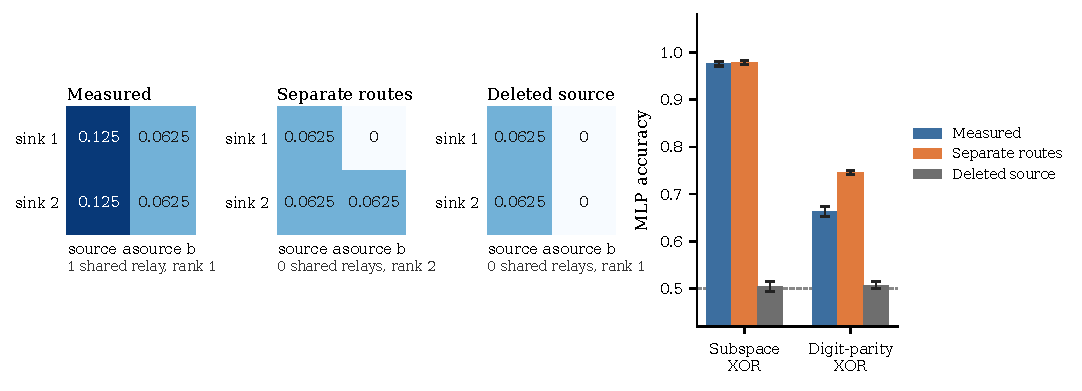
\includegraphics[width=\textwidth]{figures/transfer_readout.pdf}
\caption{Source-to-sink transfers after two rounds of incoming-neighbor averaging, and the MLP trained on the sink state. The two edits match the measured graph in degree sequence, module-pair counts, and edge count. Only the measured graph has a relay used by both sources. Error bars are percentile bootstrap intervals over ten seeds. The dashed line is chance.}
\label{fig:main}
\end{figure*}

\begin{figure}[t]
\centering
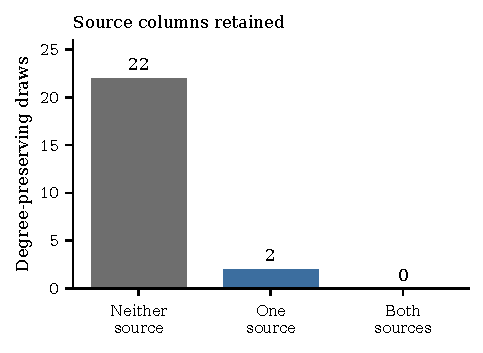
\includegraphics[width=0.92\linewidth]{figures/degree_support.pdf}
\caption{Source columns of $T$ retained by 24 degree-preserving rewires of the measured graph, each with $10\times 3{,}072$ swaps. No draw retains both sources.}
\label{fig:degree}
\end{figure}

\subsection{What the degree-preserving null retains}
\label{sec:nullresult}

Figure~\ref{fig:degree} is the degree-preserving ensemble.
All 24 draws match both degree sequences.
None matches the module-pair histogram of the measured graph.
Twenty-two draws retain neither source column.
Two retain exactly one.
None retains both.
A comparison of the measured graph against this null, on either XOR, contrasts a graph that carries both inputs with a graph that does not.
The accuracy gap that follows is the gap predicted by a deleted column.
Section~\ref{sec:routes} asks the other question, at a budget where degree-matched draws still carry both inputs.

The module-matched pair is that other comparison.
Separate routes and deleted source have the same degrees, the same modules, the same edge count, and no shared relay.
The MLP gap between them is the gap in Section~\ref{sec:split}.
Degree matching without a source-column check would have put these two graphs in one control bin.
On digit parity their accuracies are $0.746$ and $0.506$.

\subsection{What would have been misread}
\label{sec:misread}

Three summaries of the same runs give three different stories.
The subspace means say that the measured wiring and a relay-deleting edit are equivalent, near $0.98$, and that a second edit is at chance.
A motif count says the opposite of the digit-parity order: the only graph that keeps the shared relay is the middle performer, not the best.
A degree-preserving null says the measured wiring is special, because the null loses, while omitting that the null has thrown away the inputs.
The transfer distinguishes the three graphs, and it distinguishes the null from all three.
Reporting $T$, or at least the support and the rank of its columns, would have blocked each of those readings.

The direction of the digit-parity result is also easy to overstate.
The separate-routes graph is better than the measured subgraph for this readout and these two neurons.
It is one edit, on one sparsification, of one route chosen by a search rule.
It is not a claim that randomizing fly visual synapses improves vision.
It is evidence that the presence of the shared relay was not the quantity the MLP used.


\section{Degree matching at two budgets}
\label{sec:routes}

The ensemble in Figure~\ref{fig:degree} uses $10\times 3{,}072$ swaps.
A two-hop route rarely survives that budget, so the ensemble cannot ask whether degree is enough among graphs that still carry both inputs.
Holding the two-hop edges fixed does not answer that question either.
On the first three relays from the rule in Section~\ref{sec:graph}, 11 of 12 protected draws reproduce $T$ exactly, and the MLP reproduces the measured score because training uses $T$.
The twelfth, on the third route, changes one entry from $0.0625$ to $0.125$ and moves parity from $0.710$ to $0.700$.
The six draws that leave those edges free score $0.503$.
Five have a zero transfer.
The sixth keeps one column, and its six seed scores are the same chance vector.
These runs repeat a transfer.
They are not twelve wirings with different inputs.

The budget has to be short enough that both columns still occur, and long enough that $T$ is no longer the measured one.
Twelve degree-preserving rewires were drawn at each of seven lengths, from 154 swaps to $30{,}720$, and support was recorded before any accuracy at those lengths was computed.
Both columns remain in 11 of 12 draws at 154 and at 307 swaps, in 4 of 12 at 768, in 1 of 12 at $3{,}072$, and in none of 12 at $1{,}536$, $6{,}144$, and $30{,}720$.
The archived 24 draws at $30{,}720$ swaps, with seeds $50{,}000$ through $50{,}023$, agree with Figure~\ref{fig:degree}: 22 retain neither column and two retain one.
Every draw matches the in-degree and the out-degree of each neuron.
None matches the module-pair histogram.

The length used for the readout is the shortest one at which both columns occur in at least 8 of 12 draws and fewer than half the transfers equal the measured transfer.
That length is 307 swaps.
Eleven draws keep both columns: five have rank 2 and six have rank 1.
Three of those rank-1 draws copy the measured transfer.
The remaining draw deletes a column and also has rank 1.
The ten-seed MLP of Section~\ref{sec:tasks}, retrained on these transfers, scores digit parity between $0.715$ and $0.727$ on the five rank-2 draws and between $0.646$ and $0.673$ on the six rank-1 draws that keep both columns.
The deleted column scores $0.506$.
The separate-routes and deleted-source transfers, scored in the same run, give $0.746$ and $0.506$, and the measured transfer gives $0.663$.
Two of the rank-2 transfers occur twice, so the five rank-2 scores come from three maps, at $0.715$, $0.722$, and $0.727$.
Each of those maps lies above every rank-1 map in the twelve.
Degree matching does not put these graphs in one bin.
Rank does.
Figure~\ref{fig:ensemble} shows the survival curve and the twelve scores.

Digit class, scored on the three measured routes, still asks for less than parity.
Accuracy is $0.959$, $0.939$, and $0.985$ with both columns, and $0.099$ with a zero transfer.
A transfer that passes only the upper half scores $0.940$, only the lower half scores $0.895$, and the one-column rewire scores $0.878$.
One half of the digit is enough for most of that classification.
Parity is the task that separates rank 2 from rank 1 once both columns are present.

\begin{figure}[t]
\centering
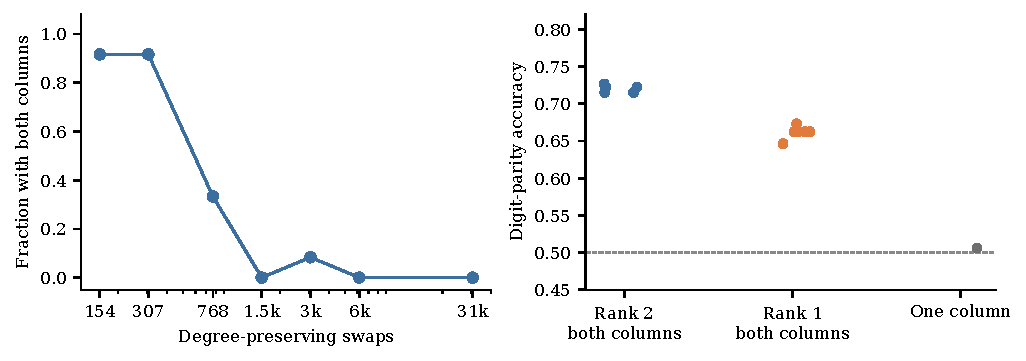
\includegraphics[width=\linewidth]{figures/ensemble.pdf}
\caption{Degree-preserving rewires of the audited route. Left: fraction of 12 draws that keep both source columns. Right: ten-seed digit-parity accuracy at 307 swaps. Points that share a transfer share a score.}
\label{fig:ensemble}
\end{figure}

\section{Discussion}
\label{sec:discussion}

A null states a hypothesis by stating what it preserves.
If the hypothesis is that in- and out-degree are enough to explain a two-input readout, the null has to be capable of carrying both inputs.
At ten swaps per edge it is not: none of the 24 draws keeps both columns.
At 307 swaps it is.
Eleven of twelve draws keep both columns, the transfer is usually no longer the measured one, and digit parity still splits by rank, $0.715$--$0.727$ against $0.646$--$0.673$.
The degree sequence is the same on both sides of that split.
The result sits next to Park's finding that standard nulls rewrite the routes a task can use \cite{park2026}.
There the nulls added one-step shortcuts the connectome did not have.
Here the long null removes two-hop inputs, and the short null keeps the inputs while changing their rank.
In both cases a gap against an unstratified degree null is not yet a difference beyond degree.

The same standard does not by itself overturn a published flyvis or Kenyon-cell result.
Dhiman's mask multiplies learned and fixed weights. It does not average incoming neighbors, and the reported endpoints are early loss and mean activity on a motion stimulus \cite{dhiman2026}.
Correig-Fraga and colleagues learn scalar gains on a whole-brain graph and read Kenyon cells \cite{correig2026}.
Liu's flips come from changing how physiology is assigned \cite{liu2026}.
None of those operators is Equation~\eqref{eq:W}.
What transfers is the reporting requirement.
A degree match, a motif count, or a cost match should be accompanied by the source support of the propagator that was actually run, on the neurons the task reads.
Where that support differs across the conditions being compared, the accuracy table is not yet a wiring result.

Two boundaries belong with that requirement.
The tasks use two selected neurons as sources and an XOR as the label.
A distributed visual code, written across a retinal array and read from a large population, can remain solvable after any single pair of columns has been damaged.
We also did not refit an optic-flow model or an eye-to-Kenyon-cell model.
The MLP result says that, for this averaging rule and this route, column support and column rank order the executed readout, and the usual certificates do not.

Mean aggregation already predicts that a larger in-degree shrinks a task synapse \cite{xu2019gin}.
The graphs here all have the same degree sequence, so that prediction does not choose among them.
The quantity that does choose is whether the two-hop routes that survive the swaps still span both sources, and whether those routes land in one sink direction or in two.
That check is a few matrix columns once $W$ is built.
It is cheaper than the training run, and on this evidence it is the control the training run is sensitive to.

\section*{LLM Usage Statement}
A coding assistant was used for drafting and for algebra and plotting checks.
Naming a non-public assistant configuration would identify the authors, so the description stays generic.
The graph files, the MLP runs, and the degree-preserving ensemble were executed locally in PyTorch 2.13 on Apple MPS.
Numbers in the paper were taken from those outputs.
The authors reviewed the manuscript and are responsible for its claims.

{\small
\bibliographystyle{ieeenat_fullname}
\bibliography{references}
}

\end{document}
